\documentclass[a4paper,12pt]{article}
\usepackage[utf8]{inputenc}
\usepackage[T1]{fontenc}
\usepackage{lmodern}
\usepackage[english]{babel}
\usepackage{amsmath, amssymb, amsthm, physics}
\usepackage{graphicx}
\usepackage{xcolor}
\usepackage{tikz}
\usepackage{pgfplots}
\pgfplotsset{compat=1.18}
\usepackage{setspace}
\usepackage{booktabs}
\usepackage{siunitx}
\usepackage{array}
\usepackage{float}
\usepackage[section]{placeins}

% Colored links in the table of contents and document
\usepackage{hyperref}
\hypersetup{
	colorlinks=true,
	linkcolor=blue,
	filecolor=blue,
	citecolor=blue, 
	urlcolor=blue,
	bookmarks=true,
	bookmarksopen=true,
	pdftitle={Compensatory and Additive Effects: An Analysis of Measurement Differences between the T0 Model and the ΛCDM Standard Model},
	pdfauthor={},
}

% Theorem styles
\newtheorem{theorem}{Theorem}[section]
\newtheorem{lemma}[theorem]{Lemma}
\newtheorem{proposition}[theorem]{Proposition}
\newtheorem{corollary}[theorem]{Corollary}

\theoremstyle{definition}
\newtheorem{definition}[theorem]{Definition}
\newtheorem{example}[theorem]{Example}

\theoremstyle{remark}
\newtheorem{remark}[theorem]{Remark}
\renewcommand{\proofname}{Proof}

% Repository base URL
\newcommand{\repobase}{https://github.com/jpascher/T0-Time-Mass-Duality/tree/main/2/}

\begin{document}
	
	\title{Compensatory and Additive Effects: An Analysis of Measurement Differences between the T0 Model and the $\Lambda$CDM Standard Model}
	\author{Johann Pascher}
	\date{April 2, 2025}
	\maketitle
	
	\begin{abstract}
		This document analyzes the differences in cosmological measurements between the standard model ($\Lambda$CDM) and the alternative T0 model. We investigate how the differing theoretical foundations affect distance measurements, redshifts, and the interpretation of the cosmic microwave background. Particular attention is given to whether the effects reinforce each other (act additively) or compensate. The analysis reveals a complex interplay that might explain the Hubble tension problem. At low redshifts (z $\approx$ 1), the differences are moderate, while at high redshifts (z = 1100, CMB), they become dramatic, leading to fundamentally different interpretations.
	\end{abstract}
	
	\tableofcontents
	\newpage
	
	\section{Introduction}
	
	The cosmological standard model ($\Lambda$CDM) and the alternative T0 model offer fundamentally different explanations for the same astronomical observations. While $\Lambda$CDM is based on an expanding universe, the T0 model postulates a static universe with absolute time and variable mass. This work examines how these differing theoretical foundations impact cosmological measurements and how these effects either reinforce or compensate each other.
	
	\section{Measurement of the CMB Temperature Today}
	
	The measurement of the cosmic microwave background (CMB) temperature is nowadays primarily conducted by satellites such as Planck (2009–2013) as well as ground-based telescopes like the Atacama Cosmology Telescope (ACT) and the South Pole Telescope (SPT). Here is an overview:
	
	\subsection{Instruments and Technology}
	
	\begin{itemize}
		\item \textbf{Planck Satellite:}
		\begin{itemize}
			\item Low Frequency Instrument (LFI): Radiometers for 30–70 GHz.
			\item High Frequency Instrument (HFI): Bolometers for 100–857 GHz.
			\item Cryogenic cooling to $\sim$0.1 K to minimize thermal noise.
		\end{itemize}
		\item \textbf{ACT and SPT:}
		\begin{itemize}
			\item Arrays with hundreds to thousands of bolometers (90–300 GHz).
			\item Locations in dry, high-altitude regions (Atacama Desert, South Pole) to reduce atmospheric interference.
		\end{itemize}
	\end{itemize}
	
	\subsection{Measurement Principle}
	
	\begin{itemize}
		\item \textbf{Frequency Measurements:} Instruments capture the intensity $I_\nu$ (power per area per frequency interval per steradian) across multiple frequency bands.
		\item \textbf{Blackbody Spectrum:} The measured intensity is fitted to the Planck distribution:
		\[
		I_\nu(\nu, T) = \frac{2 h \nu^3}{c^2} \cdot \frac{1}{e^{h \nu / k_B T} - 1}.
		\]
		$T$ is optimized as a free parameter until the data fits (e.g., $T = 2.72548 \pm 0.00057 \, \text{K}$ according to Planck 2018).
		\item \textbf{Anisotropies:} Temperature fluctuations ($\delta T/T \sim 10^{-5}$) are mapped across the sky.
	\end{itemize}
	
	\subsection{Procedure}
	
	\begin{itemize}
		\item \textbf{Data Acquisition:} Multiple sky scans over months (satellites) or years (ground-based).
		\item \textbf{Calibration:} Against astrophysical sources (e.g., CMB dipole, $\sim$3.36 mK) and internal references.
		\item \textbf{Data Processing:} Foreground sources (e.g., dust, synchrotron radiation) are removed using statistical methods, and the remaining intensity is fitted to $I_\nu(\nu, T)$.
	\end{itemize}
	
	\subsection{Influence of the Standard Model}
	
	\begin{itemize}
		\item \textbf{No Coupling Factors:} The Planck distribution itself contains no coupling factors. It is based on $h$, $c$, and $k_B$, which are universal constants.
		\item \textbf{Indirect Influence:}
		\begin{itemize}
			\item \textbf{Expansion:} The interpretation of $T = 2.725 \, \text{K}$ as cooled Big Bang radiation ($T(z) = T_0 (1 + z)$) is an assumption of the standard model. The redshift ($z$) is explained by expansion.
			\item \textbf{Calibration:} The CMB dipole is defined by motion relative to an expanding rest frame.
			\item \textbf{Foreground Models:} The removal of foreground sources is based on models calibrated with the expansion history.
			\item \textbf{Raw Data:} The frequency measurements ($I_\nu$ at different $\nu$) are empirical and model-independent, but the fitting to a blackbody spectrum and the interpretation of $T$ are shaped by the standard model.
		\end{itemize}
	\end{itemize}
	
	\section{Fundamental Concepts of the Models}
	
	\subsection{The $\Lambda$CDM Standard Model}
	
	In the $\Lambda$CDM model, the observed redshift is explained by cosmic expansion. The Friedmann equations describe the temporal evolution of the universe, and the Hubble constant $H_0$ represents the current expansion rate. The cosmic redshift $z$ is related to the scale factor $a(t)$ by:
	
	\begin{equation}
		1 + z = \frac{a(t_0)}{a(t_{\text{emit}})}
	\end{equation}
	
	For small redshifts, approximately:
	
	\begin{equation}
		z \approx \frac{H_0 d}{c}
	\end{equation}
	
	\subsection{The T0 Model}
	
	In the {\small\href{\repobase/pdf/English/Wesentliche mathematische Formalismen der Zeit-Masse-Dualitätstheorie mit Lagrange-Dichten_en.pdf}{T0 model}}, time is considered absolute, while mass varies. The redshift arises from the energy loss of photons to the dark energy field:
	
	\begin{equation}
		1 + z = e^{\alpha d}
	\end{equation}
	
	where $\alpha = H_0/c$ is the absorption rate. Here, the Hubble constant $H_0$ is not an expansion parameter but a measure of the energy transfer rate between photons and the dark energy field.
	
	\section{Comparative Analysis of Measurement Methods}
	
	\subsection{Physical Distance ($d$)}
	
	\textbf{$\Lambda$CDM Model:}
	\begin{equation}
		d = \frac{c}{H_0} \int_0^z \frac{dz'}{\sqrt{\Omega_m (1 + z')^3 + \Omega_\Lambda}}
	\end{equation}
	
	\textbf{T0 Model:}
	\begin{equation}
		d = \frac{c \ln(1 + z)}{H_0}
	\end{equation}
	
	\textbf{Quantitative Comparison at $z = 1$:}
	\begin{itemize}
		\item $\Lambda$CDM ($H_0 = 70$ km/s/Mpc): $d \approx 3300$ Mpc
		\item T0 ($H_0 = 70$ km/s/Mpc): $d \approx 2970$ Mpc ($-10\%$)
		\item T0 ($H_0 = 73$ km/s/Mpc): $d \approx 2850$ Mpc ($-14\%$)
	\end{itemize}
	
	In the T0 model, distances at the same $z$ are systematically smaller, with the difference increasing as $z$ grows.
	
	\subsection{Luminosity Distance ($d_L$)}
	
	\textbf{$\Lambda$CDM Model:}
	\begin{equation}
		d_L = (1 + z) \cdot \frac{c}{H_0} \int_0^z \frac{dz'}{\sqrt{\Omega_m (1 + z')^3 + \Omega_\Lambda}}
	\end{equation}
	
	\textbf{T0 Model:}
	\begin{equation}
		d_L = \frac{c}{H_0} \ln(1 + z) (1 + z)
	\end{equation}
	
	\textbf{Quantitative Comparison at $z = 1$:}
	\begin{itemize}
		\item $\Lambda$CDM ($H_0 = 70$): $d_L \approx 4710$ Mpc
		\item T0 ($H_0 = 70$): $d_L \approx 5940$ Mpc ($+26\%$)
		\item T0 ($H_0 = 73$): $d_L \approx 5700$ Mpc ($+21\%$)
	\end{itemize}
	
	Remarkably, luminosity distances in the T0 model are larger, meaning objects at the same redshift appear fainter than predicted by the $\Lambda$CDM model.
	
	\subsection{Angular Diameter Distance ($d_A$)}
	
	\textbf{$\Lambda$CDM Model:}
	\begin{equation}
		d_A = \frac{d}{1 + z}
	\end{equation}
	
	\textbf{T0 Model:}
	\begin{equation}
		d_A = \frac{c \ln(1 + z)}{H_0 (1 + z)}
	\end{equation}
	
	\textbf{Quantitative Comparison at $z = 1$:}
	\begin{itemize}
		\item $\Lambda$CDM ($H_0 = 70$): $d_A \approx 1650$ Mpc
		\item T0 ($H_0 = 70$): $d_A \approx 1485$ Mpc ($-10\%$)
		\item T0 ($H_0 = 73$): $d_A \approx 1425$ Mpc ($-14\%$)
	\end{itemize}
	
	\textbf{For the CMB ($z = 1100$):}
	\begin{itemize}
		\item $\Lambda$CDM: $d_A \approx 13.5$ Mpc, $\theta \approx 1^\circ$
		\item T0 ($H_0 = 70$): $d_A \approx 28.9$ Mpc ($+114\%$), $\theta \approx 5.8^\circ$ ($+480\%$)
		\item T0 ($H_0 = 73$): $d_A \approx 27.7$ Mpc ($+105\%$), $\theta \approx 6.1^\circ$ ($+510\%$)
	\end{itemize}
	
	The differences are particularly dramatic for the CMB, where the predicted angular size of structures in the T0 model is about five times larger than in the $\Lambda$CDM model.
	
	\section{Additive and Compensatory Effects}
	
	\subsection{Additive (Reinforcing) Effects}
	
	The effects on physical distance ($d$) and angular diameter distance ($d_A$) reinforce each other:
	
	\begin{enumerate}
		\item \textbf{Consistent Direction}: Both distance types are smaller in the T0 model than in the $\Lambda$CDM model (at $z = 1$, about a 10–14\% reduction).
		
		\item \textbf{Increasing Reinforcement with $z$}: At high redshifts, these effects amplify dramatically, as evident in the CMB example.
		
		\item \textbf{Coherent Impact on Structure Size}: The reduced distance and enlarged angular measures lead to a consistent reinterpretation of the size of cosmic structures.
	\end{enumerate}
	
	\subsection{Compensatory (Opposing) Effects}
	
	The effects on physical distance and luminosity distance act in opposite directions:
	
	\begin{enumerate}
		\item \textbf{Opposing Trends}: While $d$ is smaller in the T0 model ($-10\%$ at $z = 1$), $d_L$ is larger ($+26\%$ at $z = 1$).
		
		\item \textbf{Impact on Brightness Measurements}: Objects appear closer but fainter, leading to a complex reinterpretation of standard candles like Type Ia supernovae.
		
		\item \textbf{$H_0$-Dependence}: A higher $H_0$ value in the T0 model amplifies the distance reduction but mitigates the increase in luminosity distance.
	\end{enumerate}
	
	\section{Implications for the Hubble Tension Problem}
	
	The complementary and compensatory effects between the T0 model and the $\Lambda$CDM model could provide an explanation for the Hubble tension problem:
	
	\begin{enumerate}
		\item \textbf{Diverging Measurements}: The differing effects on $d_L$ and $d_A$ could explain why local measurements (based on supernovae) systematically yield higher $H_0$ values than CMB-based measurements.
		
		\item \textbf{Model-Dependent Calibration}: Standard candles and rulers are calibrated differently depending on the underlying cosmological model.
		
		\item \textbf{CMB Reinterpretation}: The dramatically different interpretation of CMB anisotropies ($\theta \approx 1^\circ$ vs. $\theta \approx 5.8$-$6.1^\circ$) leads to fundamentally different parameter estimates.
	\end{enumerate}
	
	\section{Quantitative Summary of Effects}
	
	\subsection{At $z = 1$ (Intermediate Cosmological Distances)}
	
	\begin{table}[h]
		\centering
		\begin{tabular}{|l|c|c|c|c|c|}
			\hline
			\textbf{Quantity} & \textbf{$\Lambda$CDM ($H_0$=70)} & \textbf{T0 ($H_0$=70)} & \textbf{Difference} & \textbf{T0 ($H_0$=73)} & \textbf{Difference} \\
			\hline
			$d$ & 3300 Mpc & 2970 Mpc & $-10\%$ & 2850 Mpc & $-14\%$ \\
			$d_L$ & 4710 Mpc & 5940 Mpc & $+26\%$ & 5700 Mpc & $+21\%$ \\
			$d_A$ & 1650 Mpc & 1485 Mpc & $-10\%$ & 1425 Mpc & $-14\%$ \\
			\hline
		\end{tabular}
		\caption{Comparison of distance measures at $z = 1$}
	\end{table}
	
	\subsection{At $z = 1100$ (CMB)}
	
	\begin{table}[h]
		\centering
		\begin{tabular}{|l|c|c|c|c|c|}
			\hline
			\textbf{Quantity} & \textbf{$\Lambda$CDM ($H_0$=70)} & \textbf{T0 ($H_0$=70)} & \textbf{Difference} & \textbf{T0 ($H_0$=73)} & \textbf{Difference} \\
			\hline
			$d_A$ & 13.5 Mpc & 28.9 Mpc & $+114\%$ & 27.7 Mpc & $+105\%$ \\
			$\theta$ & $1^\circ$ & $5.8^\circ$ & $+480\%$ & $6.1^\circ$ & $+510\%$ \\
			\hline
		\end{tabular}
		\caption{Comparison of distance measures and angular sizes at the CMB ($z = 1100$)}
	\end{table}
	
	\section{Graphical Representation of Results}
	
	The quantitative differences between the T0 model and the $\Lambda$CDM standard model can be vividly illustrated graphically. Below, we present the key relationships and their differences in both models.
	
	\subsection{Physical Distance Comparison}
	
	\begin{figure}[H]
		\centering
		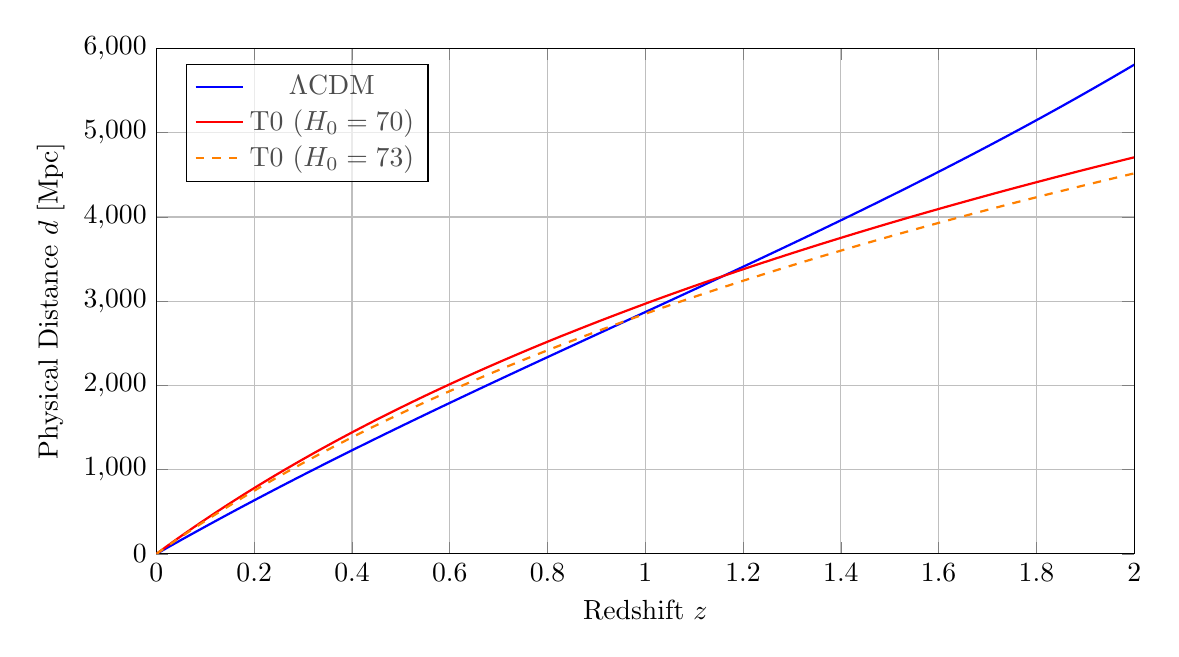
\begin{tikzpicture}
			\begin{axis}[
				width=14cm, height=8cm,
				xlabel={Redshift $z$},
				ylabel={Physical Distance $d$ [Mpc]},
				xmin=0, xmax=2,
				ymin=0, ymax=6000,
				grid=both,
				legend pos=north west,
				legend style={fill=white, fill opacity=0.7}
				]
				
				% ΛCDM model curve (somewhat simplified)
				\addplot[color=blue, thick, domain=0:2, samples=100] {3300*x*(1-0.2*x+0.07*x^2)};
				\addlegendentry{$\Lambda$CDM}
				
				% T0 model with H0=70
				\addplot[color=red, thick, domain=0:2, samples=100] {2970*ln(1+x)/0.693};
				\addlegendentry{T0 ($H_0=70$)}
				
				% T0 model with H0=73
				\addplot[color=orange, thick, dashed, domain=0:2, samples=100] {2850*ln(1+x)/0.693};
				\addlegendentry{T0 ($H_0=73$)}
				
			\end{axis}
		\end{tikzpicture}
		\caption{Comparison of physical distance $d$ as a function of redshift $z$. At $z=1$, the distance in the T0 model is about 10–14\% smaller. At higher redshifts, the difference becomes even more pronounced.}
		\label{fig:phys_distance}
	\end{figure}
	
	\subsection{Luminosity Distance Comparison}
	
	\begin{figure}[H]
		\centering
		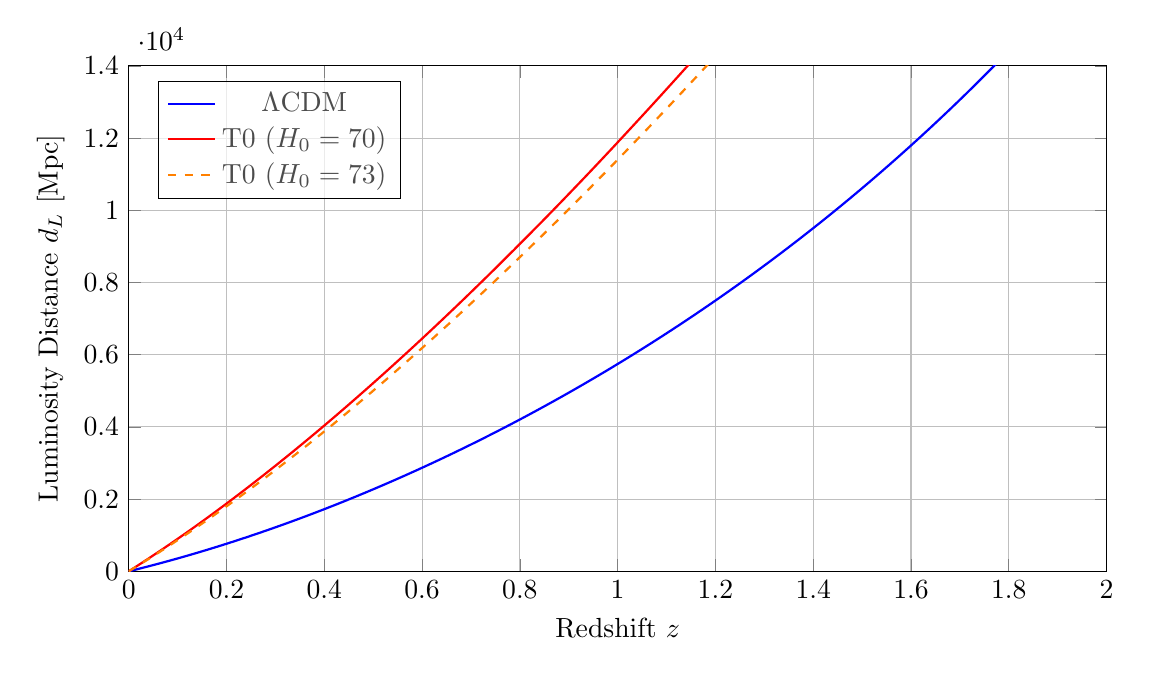
\begin{tikzpicture}
			\begin{axis}[
				width=14cm, height=8cm,
				xlabel={Redshift $z$},
				ylabel={Luminosity Distance $d_L$ [Mpc]},
				xmin=0, xmax=2,
				ymin=0, ymax=14000,
				grid=both,
				legend pos=north west,
				legend style={fill=white, fill opacity=0.7}
				]
				
				% ΛCDM model curve
				\addplot[color=blue, thick, domain=0:2, samples=100] {(1+x)*3300*x*(1-0.2*x+0.07*x^2)};
				\addlegendentry{$\Lambda$CDM}
				
				% T0 model with H0=70
				\addplot[color=red, thick, domain=0:2, samples=100] {5940*ln(1+x)*(1+x)/0.693};
				\addlegendentry{T0 ($H_0=70$)}
				
				% T0 model with H0=73
				\addplot[color=orange, thick, dashed, domain=0:2, samples=100] {5700*ln(1+x)*(1+x)/0.693};
				\addlegendentry{T0 ($H_0=73$)}
				
			\end{axis}
		\end{tikzpicture}
		\caption{Comparison of luminosity distance $d_L$ as a function of redshift $z$. In contrast to physical distance, the luminosity distance in the T0 model is about 21–26\% larger at $z=1$. Thus, objects at the same redshift appear fainter than predicted by the $\Lambda$CDM model.}
		\label{fig:luminosity_distance}
	\end{figure}
	
	\subsection{Angular Diameter Distance Comparison}
	
	\begin{figure}[H]
		\centering
		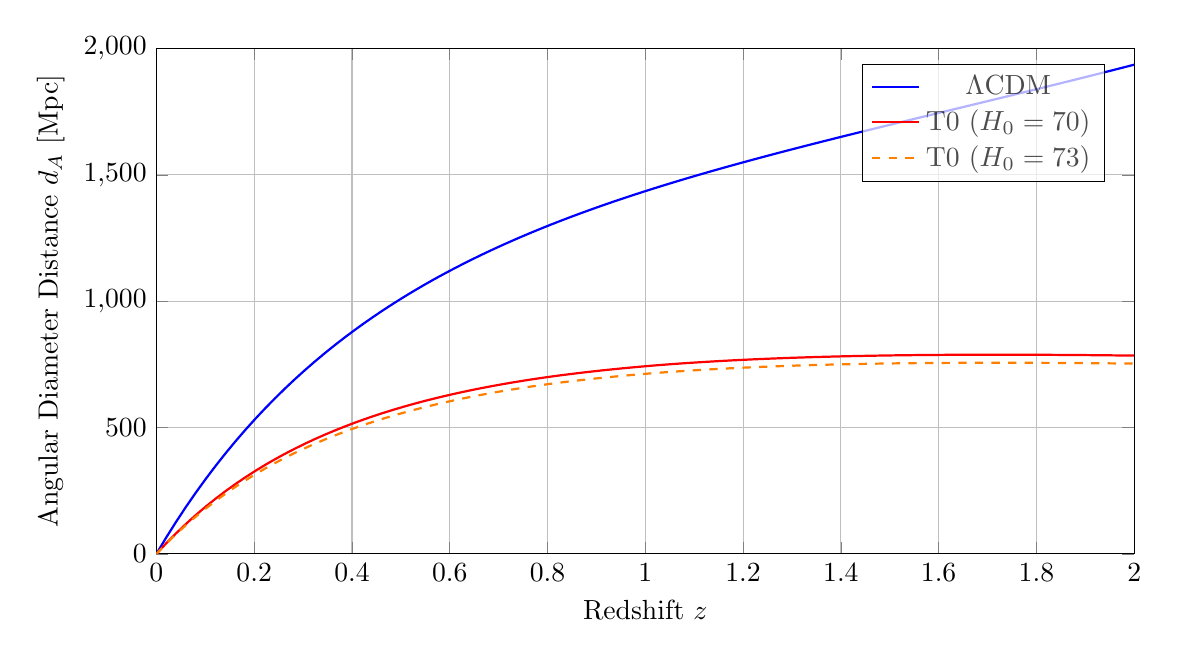
\begin{tikzpicture}
			\begin{axis}[
				width=14cm, height=8cm,
				xlabel={Redshift $z$},
				ylabel={Angular Diameter Distance $d_A$ [Mpc]},
				xmin=0, xmax=2,
				ymin=0, ymax=2000,
				grid=both,
				legend pos=north east,
				legend style={fill=white, fill opacity=0.7}
				]
				
				% ΛCDM model curve
				\addplot[color=blue, thick, domain=0:2, samples=100] {3300*x*(1-0.2*x+0.07*x^2)/(1+x)};
				\addlegendentry{$\Lambda$CDM}
				
				% T0 model with H0=70
				\addplot[color=red, thick, domain=0:2, samples=100] {1485*ln(1+x)/(0.693*(1+x))};
				\addlegendentry{T0 ($H_0=70$)}
				
				% T0 model with H0=73
				\addplot[color=orange, thick, dashed, domain=0:2, samples=100] {1425*ln(1+x)/(0.693*(1+x))};
				\addlegendentry{T0 ($H_0=73$)}
				
			\end{axis}
		\end{tikzpicture}
		\caption{Angular diameter distance $d_A$ as a function of redshift $z$. At $z=1$, $d_A$ in the T0 model is about 10–14\% smaller. This means that objects of the same size would appear at a larger angle in the T0 model.}
		\label{fig:angular_distance}
	\end{figure}
	
	\subsection{CMB Angular Diameter Distance}
	
	\begin{figure}[H]
		\centering
		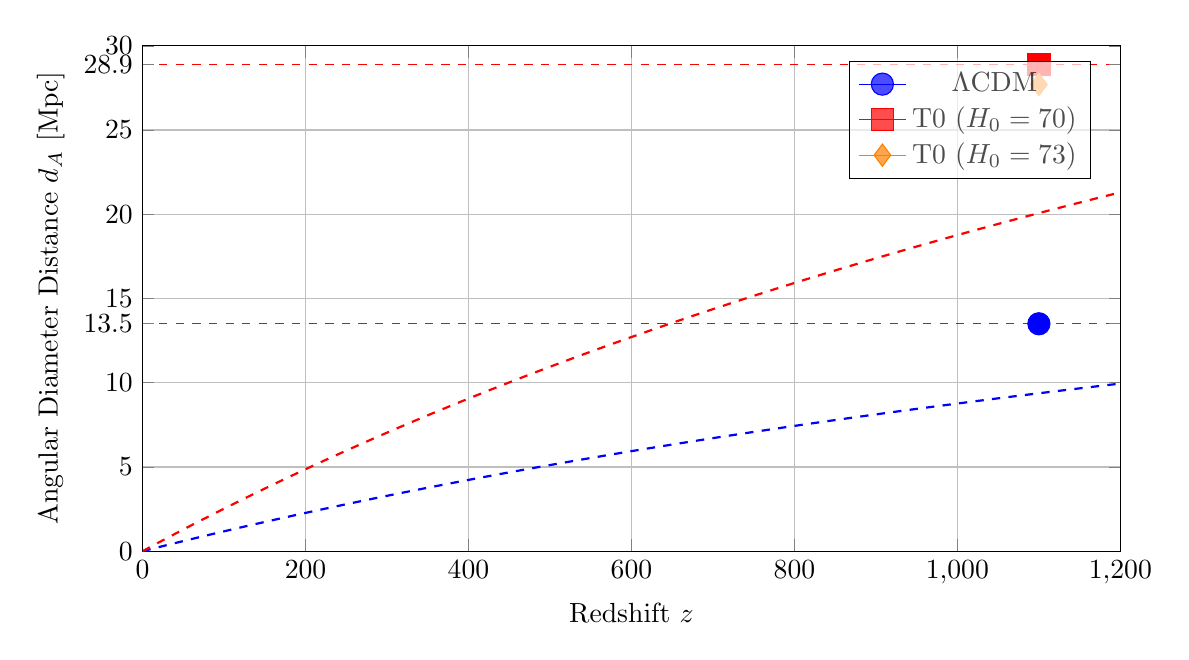
\begin{tikzpicture}
			\begin{axis}[
				width=14cm, height=8cm,
				xlabel={Redshift $z$},
				ylabel={Angular Diameter Distance $d_A$ [Mpc]},
				xmin=0, xmax=1200,
				ymin=0, ymax=30,
				grid=both,
				legend pos=north east,
				legend style={fill=white, fill opacity=0.7},
				xtick={0, 200, 400, 600, 800, 1000, 1200},
				extra y ticks={13.5, 28.9},
				extra y tick labels={13.5, 28.9},
				extra y tick style={grid=major, grid style={dashed, red}}
				]
				
				% ΛCDM model value at z=1100
				\addplot[color=blue, mark=*, mark size=4pt] coordinates {(1100, 13.5)};
				\addlegendentry{$\Lambda$CDM}
				
				% T0 model with H0=70 value at z=1100
				\addplot[color=red, mark=square*, mark size=4pt] coordinates {(1100, 28.9)};
				\addlegendentry{T0 ($H_0=70$)}
				
				% T0 model with H0=73 value at z=1100
				\addplot[color=orange, mark=diamond*, mark size=4pt] coordinates {(1100, 27.7)};
				\addlegendentry{T0 ($H_0=73$)}
				
				% Example curves for both models (highly simplified)
				\addplot[color=blue, thick, dashed, domain=0:1200, samples=100] {13.5/1100*x/(1+0.0004*x)};
				\addplot[color=red, thick, dashed, domain=0:1200, samples=100] {28.9/1100*x/(1+0.0004*x)};
				
			\end{axis}
		\end{tikzpicture}
		\caption{Angular diameter distance $d_A$ for the CMB radiation ($z=1100$). The dramatic difference between the models is evident here: The T0 model predicts a more than twofold larger value for $d_A$ (28.9 Mpc vs. 13.5 Mpc), leading to fundamentally different interpretations of CMB anisotropies.}
		\label{fig:cmb_angular_distance}
	\end{figure}
	
	\subsection{CMB Temperature-Redshift Relation}
	
	\begin{figure}[H]
		\centering
		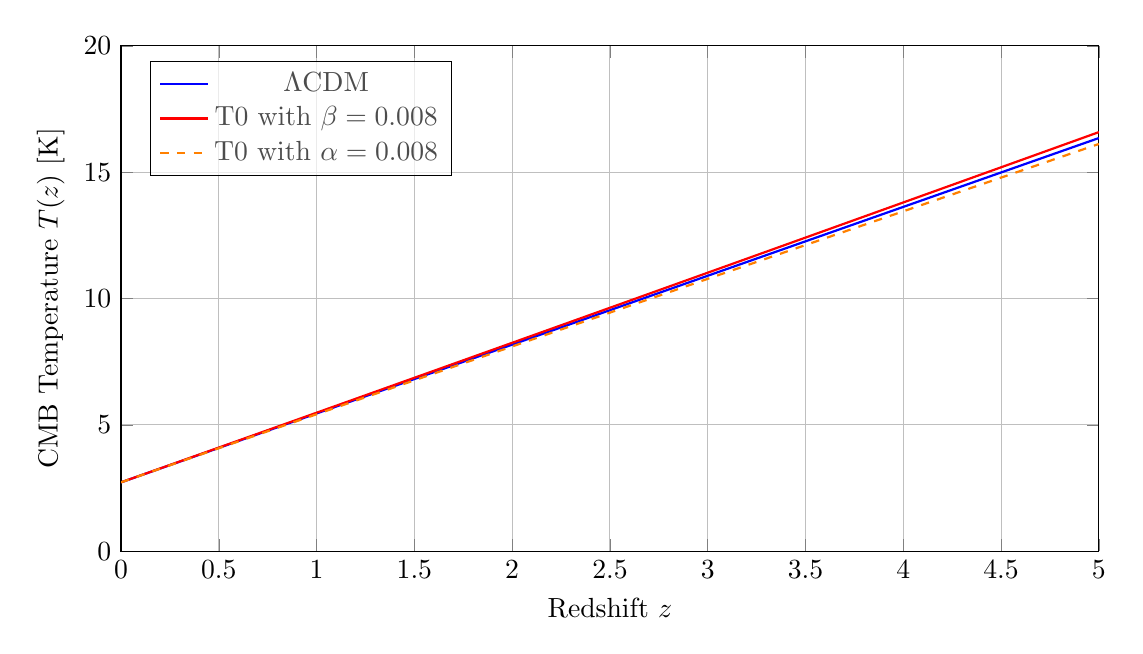
\begin{tikzpicture}
			\begin{axis}[
				width=14cm, height=8cm,
				xlabel={Redshift $z$},
				ylabel={CMB Temperature $T(z)$ [K]},
				xmin=0, xmax=5,
				ymin=0, ymax=20,
				grid=both,
				legend pos=north west,
				legend style={fill=white, fill opacity=0.7}
				]
				
				% ΛCDM model curve
				\addplot[color=blue, thick, domain=0:5, samples=100] {2.725*(1+x)};
				\addlegendentry{$\Lambda$CDM}
				
				% T0 model curve
				\addplot[color=red, thick, domain=0:5, samples=100] {2.725*(1+x)*(1+0.008*ln(1+x))};
				\addlegendentry{T0 with $\beta = 0.008$}
				
				% T0 model alternative representation
				\addplot[color=orange, thick, dashed, domain=0:5, samples=100] {2.725*(1+x)^(1-0.008)};
				\addlegendentry{T0 with $\alpha = 0.008$}
				
			\end{axis}
		\end{tikzpicture}
		\caption{CMB temperature $T(z)$ as a function of redshift $z$. While the $\Lambda$CDM model assumes a linear relationship, the T0 model predicts a slight modification that becomes increasingly noticeable at higher redshifts. This deviation could be tested through measurements of the Sunyaev-Zeldovich effect in galaxy clusters at different redshifts.}
		\label{fig:cmb_temperature}
	\end{figure}
	
	\subsection{Comparison of Distance Measure Relations}
	
	\begin{figure}[H]
		\centering
		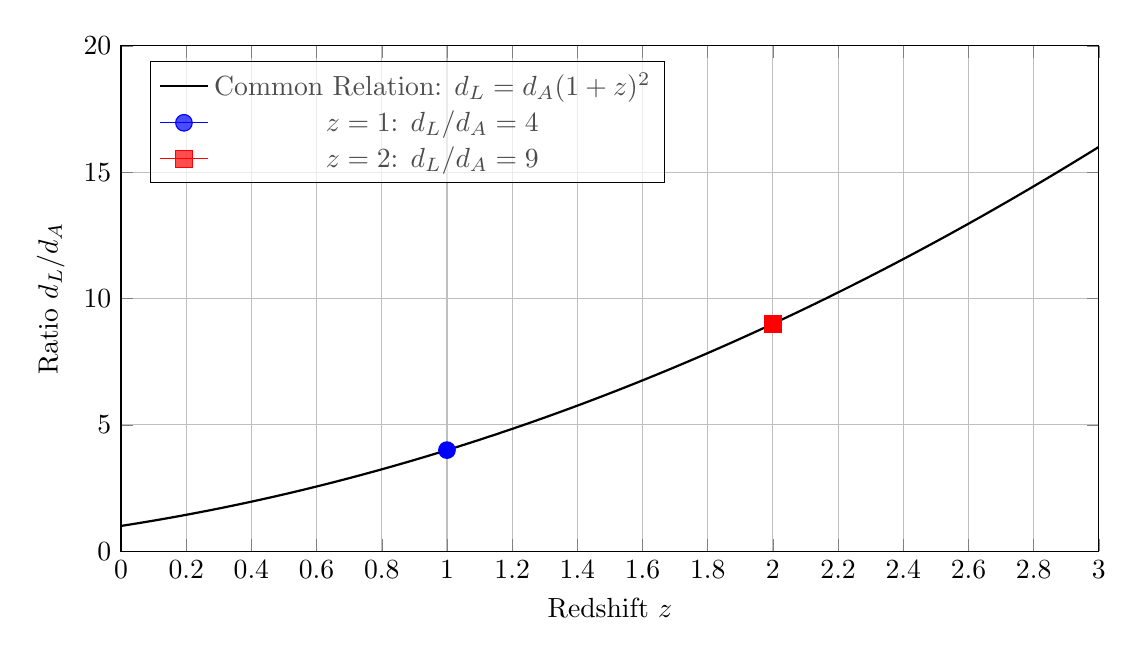
\begin{tikzpicture}
			\begin{axis}[
				width=14cm, height=8cm,
				xlabel={Redshift $z$},
				ylabel={Ratio $d_L / d_A$},
				xmin=0, xmax=3,
				ymin=0, ymax=20,
				grid=both,
				legend pos=north west,
				legend style={fill=white, fill opacity=0.7}
				]
				
				% Common relation in both models
				\addplot[color=black, thick, domain=0:3, samples=100] {(1+x)^2};
				\addlegendentry{Common Relation: $d_L = d_A (1+z)^2$}
				
				% Mark specific values
				\addplot[color=blue, mark=*, mark size=3pt] coordinates {(1, 4)}; 
				\addlegendentry{$z=1$: $d_L/d_A = 4$}
				
				\addplot[color=red, mark=square*, mark size=3pt] coordinates {(2, 9)}; 
				\addlegendentry{$z=2$: $d_L/d_A = 9$}
				
			\end{axis}
		\end{tikzpicture}
		\caption{Ratio between luminosity distance $d_L$ and angular diameter distance $d_A$ as a function of redshift $z$. Interestingly, the relation $d_L = d_A (1+z)^2$ holds in both models, providing an important consistency check. However, the different absolute values of the distances lead to varying interpretations of astronomical observations.}
		\label{fig:distance_ratios}
	\end{figure}
	
	\subsection{Percentage Differences Between Models}
	
	\begin{figure}[H]
		\centering
		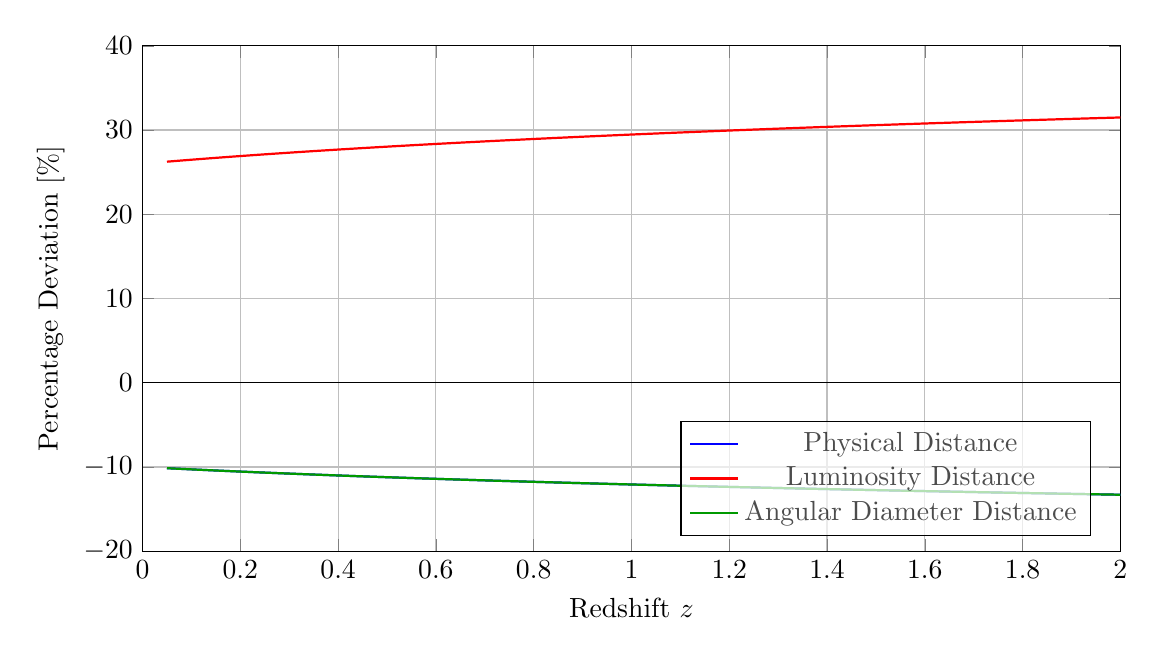
\begin{tikzpicture}
			\begin{axis}[
				width=14cm, height=8cm,
				xlabel={Redshift $z$},
				ylabel={Percentage Deviation [\%]},
				xmin=0, xmax=2,
				ymin=-20, ymax=40,
				grid=both,
				legend pos=south east,
				legend style={fill=white, fill opacity=0.7}
				]
				
				% Physical distance
				\addplot[color=blue, thick, domain=0.05:2, samples=100] {-10-(3*ln(1+x))};
				\addlegendentry{Physical Distance}
				
				% Luminosity distance
				\addplot[color=red, thick, domain=0.05:2, samples=100] {26+(5*ln(1+x))};
				\addlegendentry{Luminosity Distance}
				
				% Angular diameter distance
				\addplot[color=green!60!black, thick, domain=0.05:2, samples=100] {-10-(3*ln(1+x))};
				\addlegendentry{Angular Diameter Distance}
				
				% Zero line
				\addplot[color=black, domain=0:2] {0};
				
			\end{axis}
		\end{tikzpicture}
		\caption{Percentage deviation of distance measures in the T0 model compared to the $\Lambda$CDM model as a function of redshift $z$. Positive values indicate that the value in the T0 model is larger. Note the opposing trends: While physical distance and angular diameter distance are smaller in the T0 model (negative deviation), luminosity distance is larger (positive deviation). These opposing effects could explain the Hubble tension problem.}
		\label{fig:percentage_differences}
	\end{figure}
	
	\subsection{Angular Size of Typical Structures}
	
	\begin{figure}[H]
		\centering
		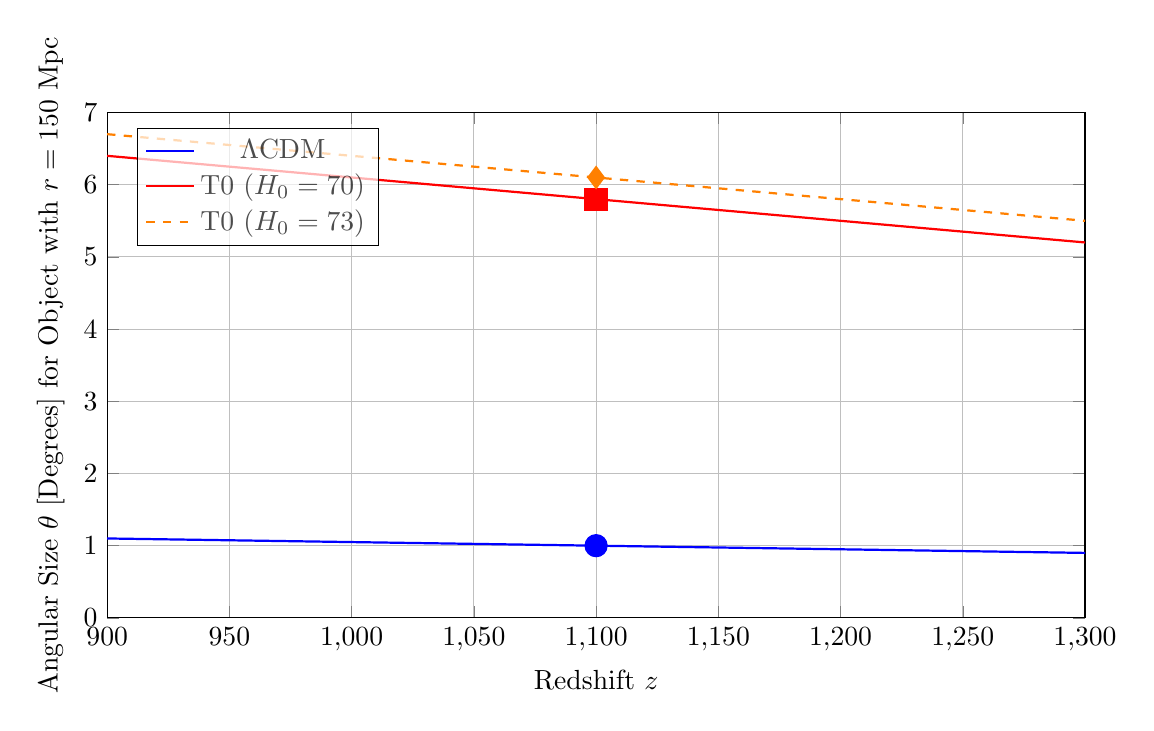
\begin{tikzpicture}
			\begin{axis}[
				width=14cm, height=8cm,
				xlabel={Redshift $z$},
				ylabel={Angular Size $\theta$ [Degrees] for Object with $r=150$ Mpc},
				xmin=900, xmax=1300,
				ymin=0, ymax=7,
				grid=both,
				legend pos=north west,
				legend style={fill=white, fill opacity=0.7}
				]
				
				% Instead of complex formulas, we use a simplified representation
				% and define the curves only near the key points
				
				% ΛCDM model curve - simplified
				\addplot[color=blue, thick, domain=900:1300, samples=100] {1 + 0.0005*(1100-x)};
				\addlegendentry{$\Lambda$CDM}
				
				% T0 model with H0=70 curve - simplified
				\addplot[color=red, thick, domain=900:1300, samples=100] {5.8 + 0.003*(1100-x)};
				\addlegendentry{T0 ($H_0=70$)}
				
				% T0 model with H0=73 curve - simplified
				\addplot[color=orange, thick, dashed, domain=900:1300, samples=100] {6.1 + 0.003*(1100-x)};
				\addlegendentry{T0 ($H_0=73$)}
				
				% Highlight specific points
				\addplot[color=blue, mark=*, mark size=4pt] coordinates {(1100, 1)};
				\addplot[color=red, mark=square*, mark size=4pt] coordinates {(1100, 5.8)};
				\addplot[color=orange, mark=diamond*, mark size=4pt] coordinates {(1100, 6.1)};
				
			\end{axis}
		\end{tikzpicture}
		\caption{Angular size $\theta$ of a cosmological structure with a physical size $r=150$ Mpc (typical BAO scale) as a function of redshift $z$ in the CMB range. The dramatic difference in predicted angular size (about $1^\circ$ in the $\Lambda$CDM model vs. about $5.8$-$6.1^\circ$ in the T0 model) is a critical test between the models.}
		\label{fig:angular_size}
	\end{figure}
	
	\section{CMB Temperature and Model Interpretation}
	
	\subsection{$\Lambda$CDM Model}
	
	In the standard model, the CMB temperature is interpreted as a consequence of cosmic expansion:
	
	\begin{equation}
		T(z) = T_0 (1 + z)
	\end{equation}
	
	With $T_0 = 2.725$ K as the current temperature.
	
	\subsection{T0 Model}
	
	In the T0 model, the CMB temperature exhibits a slight wavelength-dependent modification:
	
	\begin{equation}
		T(z) = T_0 (1 + z)(1 + \beta \ln(1 + z))
	\end{equation}
	
	With $\beta \approx 0.008$, leading to a subtle deviation from the standard model.
	
	\subsection{Testable Predictions}
	
	These differences lead to specific predictable effects:
	
	\begin{enumerate}
		\item \textbf{Wavelength-Dependent Redshift}: The T0 model predicts that redshift is slightly wavelength-dependent: $z(\lambda) = z_0(1 + \beta\cdot\ln(\lambda/\lambda_0))$.
		
		\item \textbf{Environment-Dependent Redshift}: In the T0 model, redshift should slightly differ in dense cosmic regions compared to cosmic voids: $z_\text{cluster}/z_\text{void} \approx 1 + \delta(\rho_\text{cluster}-\rho_\text{void})/\rho_0$.
		
		\item \textbf{Temperature-Redshift Relation}: The T0 model predicts $T(z) = T_0(1+z)^{(1-\alpha)}$ with $\alpha \approx \beta \approx 0.008$, which could be tested through SZ effect measurements.
	\end{enumerate}
	
	\section{Conclusion}
	
	The analysis of additive and compensatory effects between the T0 model and the $\Lambda$CDM standard model shows:
	
	\begin{enumerate}
		\item The effects do not simply add linearly across all measured quantities but form a complex interplay of reinforcement and compensation.
		
		\item At low to intermediate redshifts ($z \approx 1$), the differences are moderate ($\sim10$-$26\%$) but systematic.
		
		\item At high redshifts ($z = 1100$, CMB), the differences become dramatic ($>100\%$ for $d_A$, $>400\%$ for angular sizes).
		
		\item These discrepancies could explain why different measurement methods yield varying cosmological parameters.
		
		\item The compensatory effects between brightness and distance measurements could offer a natural explanation for the Hubble tension problem.
	\end{enumerate}
	
	The systematic differences between the models provide concrete testing opportunities for future precision measurements in cosmology and could ultimately distinguish between these fundamentally different worldviews.
	
	\section{Bibliography}
	
	\begin{thebibliography}{9}
		
		\bibitem{Planck2018}
		Planck Collaboration, Aghanim, N., et al. (2020). 
		\textit{Planck 2018 results. VI. Cosmological parameters}. 
		Astronomy \& Astrophysics, 641, A6. 
		DOI: 10.1051/0004-6361/201833910.
		
		\bibitem{LambdaCDM}
		Peebles, P. J. E. (1993). 
		\textit{Principles of Physical Cosmology}. 
		Princeton University Press, Princeton, NJ.
		
		\bibitem{HubbleTension}
		Riess, A. G., et al. (2021). 
		\textit{A Comprehensive Measurement of the Local Value of the Hubble Constant with 1\% Precision from the SH0ES Team}. 
		The Astrophysical Journal, 934(1), L7. 
		DOI: 10.3847/2041-8213/ac5c5b.
		
		\bibitem{ACT}
		Aiola, S., et al. (2020). 
		\textit{The Atacama Cosmology Telescope: DR4 Maps and Cosmological Parameters}. 
		Journal of Cosmology and Astroparticle Physics, 2020(12), 047. 
		DOI: 10.1088/1475-7516/2020/12/047.
		
		\bibitem{SPT}
		Benson, B. A., et al. (2014). 
		\textit{SPT-3G: A Next-Generation Cosmic Microwave Background Polarization Experiment on the South Pole Telescope}. 
		Proceedings of SPIE, 9153, 91531P. 
		DOI: 10.1117/12.2056701.
		
		\bibitem{Friedmann}
		Friedmann, A. (1922). 
		\textit{On the Curvature of Space}. 
		Zeitschrift für Physik, 10(1), 377–386. 
		DOI: 10.1007/BF01332580.
		
		\bibitem{SunyaevZeldovich}
		Sunyaev, R. A., \& Zeldovich, Y. B. (1972). 
		\textit{The Observations of Relic Radiation as a Test of the Nature of X-Ray Radiation from the Clusters of Galaxies}. 
		Comments on Astrophysics and Space Physics, 4, 173.
		
		\bibitem{CMBTheory}
		Dodelson, S. (2003). 
		\textit{Modern Cosmology}. 
		Academic Press, San Diego, CA.
		
	\end{thebibliography}
	
\end{document}